\documentclass[
11pt, % The default document font size, options: 10pt, 11pt, 12pt
%oneside, % Two side (alternating margins) for binding by default, uncomment to switch to one side
english, % ngerman for German
singlespacing, % Single line spacing, alternatives: onehalfspacing or doublespacing
%draft, % Uncomment to enable draft mode (no pictures, no links, overfull hboxes indicated)
%nolistspacing, % If the document is onehalfspacing or doublespacing, uncomment this to set spacing in lists to single
%liststotoc, % Uncomment to add the list of figures/tables/etc to the table of contents
%toctotoc, % Uncomment to add the main table of contents to the table of contents
parskip, % Uncomment to add space between paragraphs
%nohyperref, % Uncomment to not load the hyperref package
headsepline, % Uncomment to get a line under the header
%sectioninoneline, % Uncomment to place the section title next to the number on one line
%consistentlayout, % Uncomment to change the layout of the declaration, abstract and acknowledgements pages to match the default layout
]{report} % The class file specifying the document structure

\usepackage[utf8]{inputenc} % Required for inputting international characters
\usepackage[T1]{fontenc} % Output font encoding for international characters

\usepackage{mathpazo} % Use the Palatino font by default

\usepackage[backend=biber,style=numeric,sortcites=ynt,sorting=nyt,natbib=true]{biblatex} % Use the bibtex backend with the authoryear citation style (which resembles APA)

\addbibresource{References.bib} % The filename of the bibliography

\usepackage[autostyle=true]{csquotes} % Required to generate language-dependent quotes in the bibliography

\usepackage{mathtools, tikz}

%----------------------------------------------------------------------------------------
%	MARGIN SETTINGS
%----------------------------------------------------------------------------------------

\geometry{
	paper=a4paper, % Change to letterpaper for US letter
	inner=2.5cm, % Inner margin
	outer=2.8cm, % Outer margin
	bindingoffset=.5cm, % Binding offset
	top=1.5cm, % Top margin
	bottom=1.5cm, % Bottom margin
	%showframe, % Uncomment to show how the type block is set on the page
}

\newtheorem{theorem}{Theorem}
\newtheorem{corollary}{Corollary}[theorem]
\newtheorem{lemma}[theorem]{Lemma}
\newtheorem{definition}[theorem]{Defintion}

\title{INF5870 - Assignment 2}
\author{Zahra G. Yndestad \\ Khalil Abuawad \\ Marius E. G. Andresen \\ Christopher A. Trotter}
\date{February 2017}

\begin{document}

%----------------------------------------------------------------------------------------
%	TITLE PAGE
%----------------------------------------------------------------------------------------

\begin{titlepage}
\begin{center}

\vspace*{.06\textheight}
%{\scshape\LARGE \univname\par}\vspace{1.5cm} % University name
%\textsc{\Large Master Thesis}\\[0.5cm] % Thesis type

%\HRule \\[0.4cm] % Horizontal line
{\huge \bfseries INF5870 - Assignment 1 Report \par}\vspace{1cm} % Thesis title
%\HRule \\[1.5cm] % Horizontal line

\Large \textit{Assignment submitted in partial fulfillment of the requirements for the}
\textit{\textbf{Energy Informatics} course}  % University requirement text
\textit{at the \textbf{Institute of Informatics,}}\\
\textit{\textbf{University of Oslo}.}\\[1cm]

\Large \textit{Authors:}\\
%\vfill
\LARGE \authorname\\

\vfill


\includegraphics[scale=0.5]{uioLogo.jpg}\\[1cm]

\vfill

{\large \today}\\[4cm] % Date
%\includegraphics{Logo} % University/department logo - uncomment to place it

\vfill
\end{center}
\end{titlepage}


\frontmatter % Use roman page numbering style (i, ii, iii, iv...) for the pre-content pages

\tableofcontents % Prints the main table of contents

\pagestyle{plain} % Default to the plain heading style until the thesis style is called for the body content

\newpage

\section{Weather Data}
    Before analyzing the results from applying the machine learning techniques, we will briefly discuss the \emph{type of problem} we are attempting to solve. It will provide us with the necessary intuition for further discussion of \emph{the validity of the models} based on the data provided in the assignment. The type of problem we are concerned with is a \emph{prediction problem}. The goal of a prediction problem is to give the correct label(e.g. prediction or output) to an instance (e.g. context or input). As mentioned in \cite{predprob}, the general prediction paradigm is then
    % What model?
    
    \begin{itemize}
        \item find a representative set of $m$ instances of the problem, $u_{1},..., u_{m}$.
        \item human (the "teacher") provides the correct labels $y_{1},...,y_{m}$
        \item each ($u_{i}, y_{i}$) pair is a "labeled example"
        \item ML algorithm attempts to identify the simple hypothesis which explains the relationship between the inputs and outputs.
    \end{itemize}
    
    This latter approach lends itself well to \emph{generalization}, which is the idea of looking at $m$ examples, \emph{identifying a hypothesis}, and applying it to the next example. Identifying a hypothesis is trivial, but the challenge is that there might be infinitely many hypotheses associated with the same data, and we have to choose something, so choose the simplest one.
    
    When considering the machine learning techniques, mentioned in the assignment, they are concerned with providing examples rather than finding the actual solution, and this is done by \emph{learning} from earlier examples. It is an attempt to understand and go beyond the ability to explain something that has already been seen. Intuitively, understanding is closely related to the capability of predicting what has yet to be observed. In other words, generalization is a form of understanding.
    
    When considering the validity of the model, we have chosen to apply the model validation technique known as \emph{cross-validation}. It is a technique for assessing how the results of a statistical analysis will generalize to an \emph{independent data set}. It is mainly used in the settings where the goal is prediction, and one wants to estimate how accurately a predictive model will perform in practice. If the order of the data is important, then cross-validation might be problematic for \emph{time-series} models. We will then attempt to use an appropriate approach such as \emph{forward chaining} to validate the model.

    We will be limiting the scope of the prediction problem to only consider regression problems since the assignment limits the machine learning techniques to supervised statistical learning methods.

\section{Question 1}
    We will provide a formulation of the various models based on the data from the assignment. This includes the training data since we are considering only the model. Further, we hope to make a few statements on the validity of the model based on \emph{cross-validation}. Finally, we will provide the \emph{Root Mean Square Error}, also known as \emph{RMSE}, equation as well as the results from this equation. It will allow us to have a short discussion of the results produced from the different models.

\subsection{Linear Regression}
    The general formulation of a linear regression problem is    
    
    \begin{equation}
        y_{p} = \beta x + C.
    \end{equation}
    
    In our case the formula would be
    
    \begin{equation}
        Wind\ power_{p} = \beta \times Wind\ speed + C
    \end{equation}
    
    where $\beta = 0.1225934$ and $C = -0.08367458$, after training the model on 16080 data points from the training data. Below is a figure which represents the linear regression of the above formulation.
    
    \begin{center}
        \textbf{LR model}\\
	    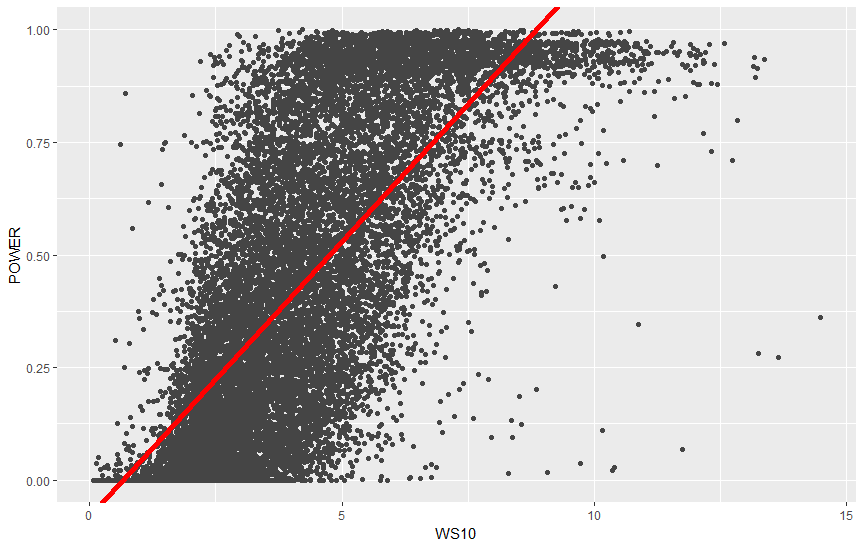
\includegraphics[scale=0.3, width=\textwidth]{figures/Rplot_LR_model.png}\\[1cm]
    \end{center}
	
	Another figure below shows the prediction of wind power from the linear regression model, where the red line is the prediction and the gray is the actual wind power. The coloring of the lines will remain the same for the other models. As for the error value, the RMSE $\approx$ 0.216. A table of the RMSE value of the different models will be presented after showing the other machine learning techniques.
    
\newpage

    \begin{center}
        \textbf{LR prediction}\\
	    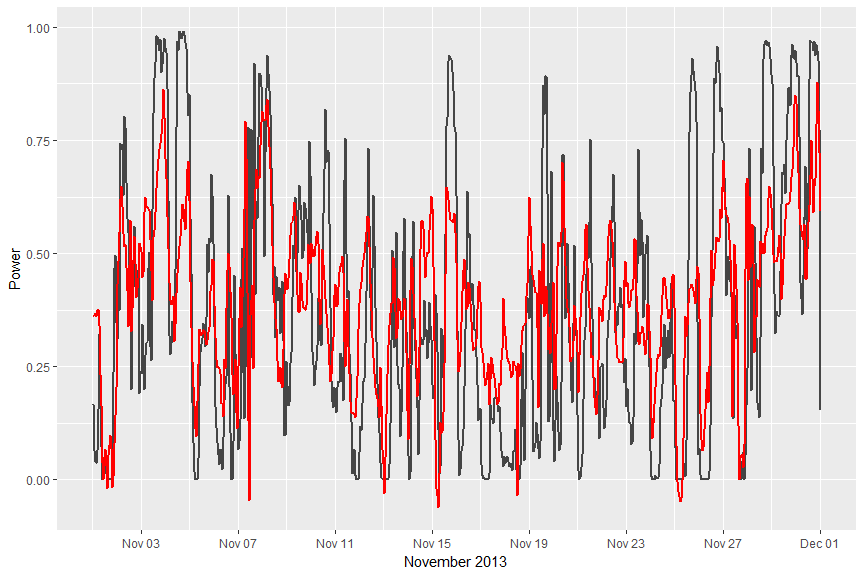
\includegraphics[scale=0.3, width=\textwidth]{figures/Rplot_LR.png}\\[1cm]
    \end{center}
    

	
\subsection{K Nearest Neighbors}
    K nearest neighbors algorithm stores all available cases and predicts the numerical target based on a similarity measure (e.g. distance function). The most common distance function is
    
    \begin{equation}
        Euclidean = \sqrt{\sum_{i=1}^{k}(x_{i} - y_{i})^{2}} .
    \end{equation}
    
    In our case the formula would be
    
    \begin{equation}
        Wind Power_{p} = \sqrt{\sum^{16080}_{i = 1}(wind\ speed_{i} - wind\ power_{i})^{2}} .
    \end{equation}
    
    Where $wind\ speed_{i}$ and $wind\ power_{i}$ refer to the corresponding columns within the training data, and 16080 is the number of data points in the training data. The optimal number of k neighbors after using \emph{cross-validation} of 10-fold is k = 23. As mentioned earlier, we will give a justification for the validity of the model after introducing the other machine learning techniques. Below is a figure which represents the optimal k nearest neighbor.

\newpage

    \begin{center}
        \textbf{KNN model}\\
	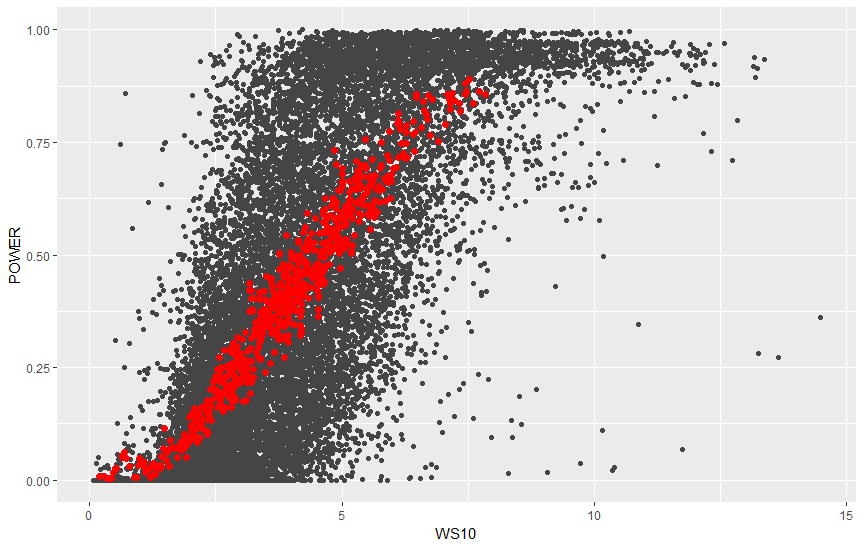
\includegraphics[scale=0.3, width=\textwidth]{figures/Rplot_KNN_model_plot.png}\\[1cm]
    \end{center}
    
    When KNN is used for regression problems the prediction is based on the mean or the median of the K-most similar instances. Furthermore, we have another figure below which shows the prediction of wind power from the KNN model. Where the coloring scheme is as mentioned before. As for the error value, the RMSE $\approx$ 0.221.
    
    \begin{center}
        \textbf{KNN prediction}\\
	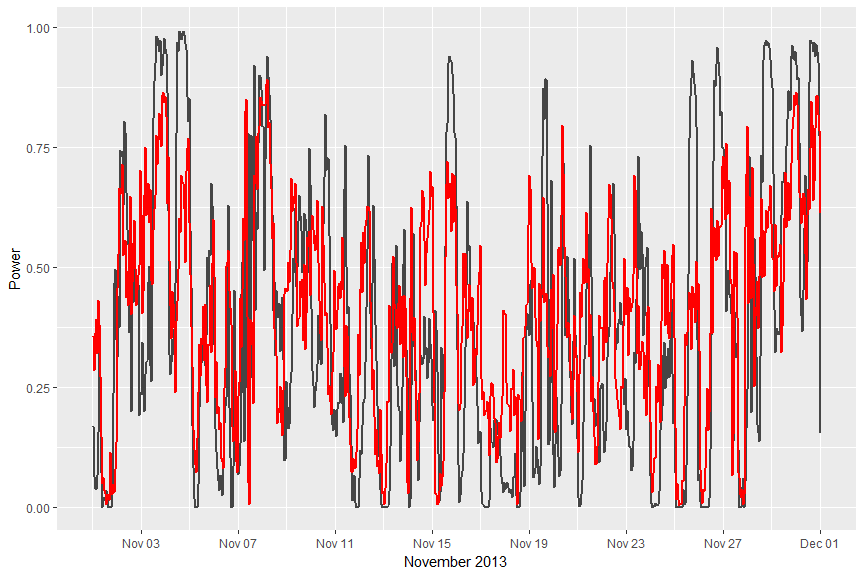
\includegraphics[scale=0.3, width=\textwidth]{figures/Rplot_KNN.png}\\[1cm]
    \end{center}
    
    
\subsection{Support Vector Machine}
    In our assignment, we will only consider the type of support vector machine used in regression problems, known as SVR. The goal is to find a function $f(x)$ that deviates from $y_{n}$ by a value no greater than $\epsilon$ for each training point x, and at the same time is as flat as possible. We are to consider the general linear regression formula as mentioned earlier.
    
    For the general linear regression function, flatness means that we wish to find a small $\beta$, which can be described by the following equation
    
    \begin{equation}
        min\ \frac{1}{2}\ \beta^2
    \end{equation}
    
    such that
    
    \begin{align*}\\[-1cm]
        y_{i} - (\beta \times x_{i} + C) \leq \epsilon \\
        (\beta \times  x_{i} + C) - y_{i} \leq \epsilon
    \end{align*}
    
     
    holds. We wish to have flatness to ensure that we avoid the over-fitting problem. Making it so that function is less sensitive to x and the change of x, as mentioned in \cite{svmForm}. When over-fitting it matches the training model, but will be a poor model for predicting new data. In our case, the epsilon would be determined by the constraints
    
    \begin{align*}\\[-1cm]
        wind\ power_{i} - (\beta \times wind\ speed_{i} + C) \leq \epsilon \\
        (\beta \times wind\ speed_{i} + C) - wind\ power_{i} \leq \epsilon .
    \end{align*}
    
    Below is first the SVR model and secondly the SVR prediction figure. First, the SVR model represents the linear formula which respects the constraints mentioned and in this case is demonstrated by using the \emph{svmRadial} method, which is available from the popular \emph{R}-library \emph{Caret}. We shall give a brief justification, at the end, for the use of \emph{svmRadial} method. Secondly, we have the figure which shows the prediction of wind power from the SVR model. The coloring scheme remains the same as the other models above. As for the error function, the RMSE $\approx$ 0.214.

\newpage

    \begin{center}
        \textbf{SVR Model}\\
    	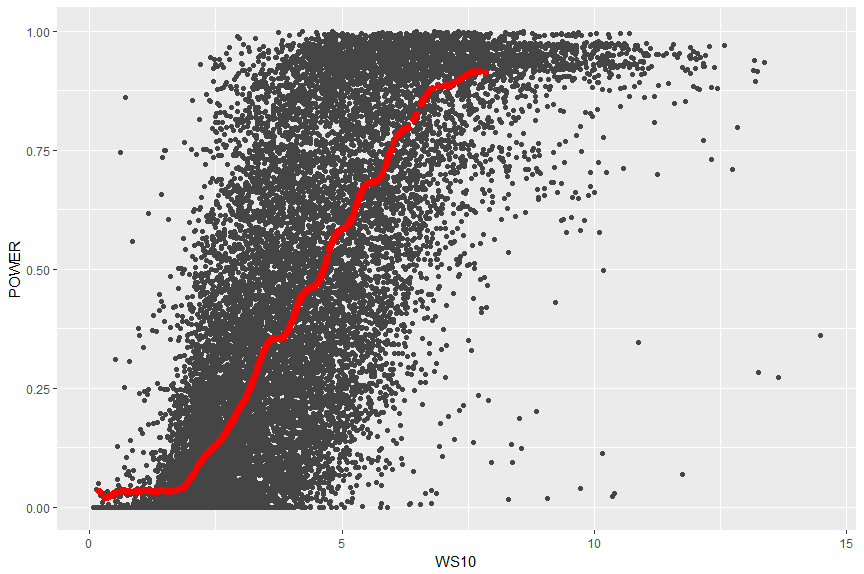
\includegraphics[scale=0.3, width=\textwidth]{figures/Rplot_SVR_model.png}\\[1cm]    
    \end{center}
    
    \begin{center}
        \textbf{SVR Prediction}\\
    	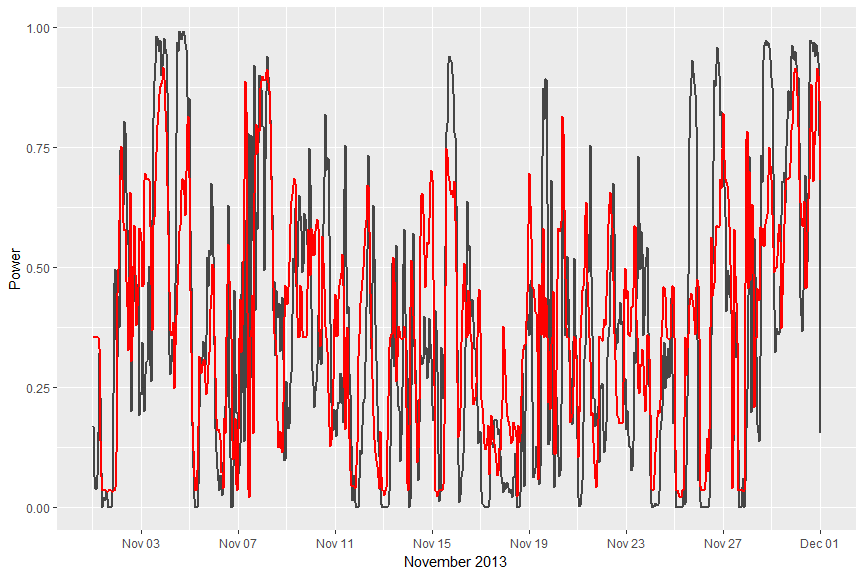
\includegraphics[scale=0.3, width=\textwidth]{figures/Rplot_SVR.png}\\[1cm]    
    \end{center}

\newpage

\subsection{Artificial Neural Network}

    The general formulation of a neural network is
    
	\begin{equation}
	    y = \sum_{i = 1}^{m}(\beta_{i}x_{i}) + \epsilon
	\end{equation}
	
	such that
	
	\begin{center}
	    \[
            f(x)= 
	        \begin{dcases}
                1 & \text{if } \sum \beta x \geq 0\\
                0 & \text{if} \sum \beta x < 0
            \end{dcases}
        \]
    \end{center}
    
    holds. This is the formulation provided from the lecture notes \cite{neuralnetForm}. Artificial Neural Network, known as ANN, suffers from the same problem as SVR which is over-fitting when considering large amounts of data. We will give a justification at the end for what may occur when over-fitting the model and discuss the validity of the model. In our case, the variable $X$ is replaced with the \emph{wind speed} in the formulation above. Besides that, everything remains the same. Below is both the ANN model and prediction figure shown in a similar fashion as SVM. As for the error function, the RMSE $\approx$ 0.216
	
	\begin{center}
	    \textbf{ANN model}\\
    	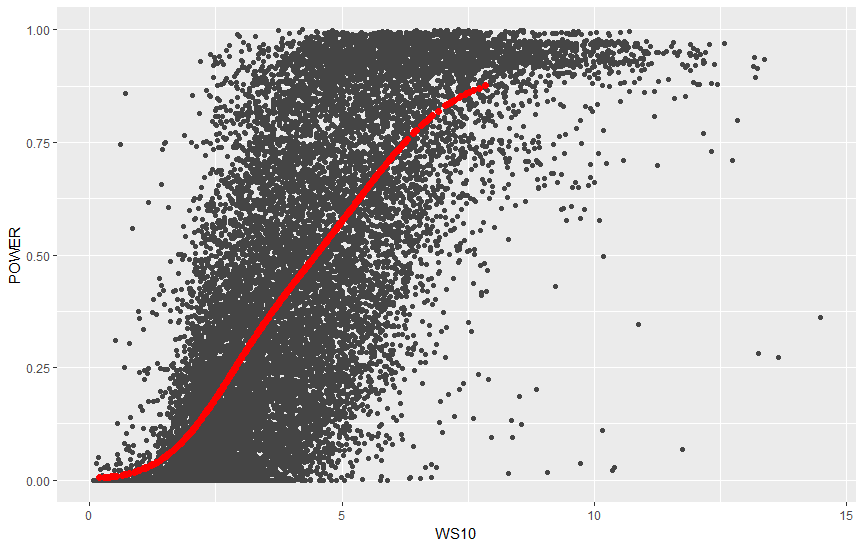
\includegraphics[scale=0.3, width=\textwidth]{figures/Rplot_ANN_model_data.png}\\[1cm]    
	\end{center}
	
\newpage
	
	\begin{center}
	    \textbf{ANN Prediction}\\
    	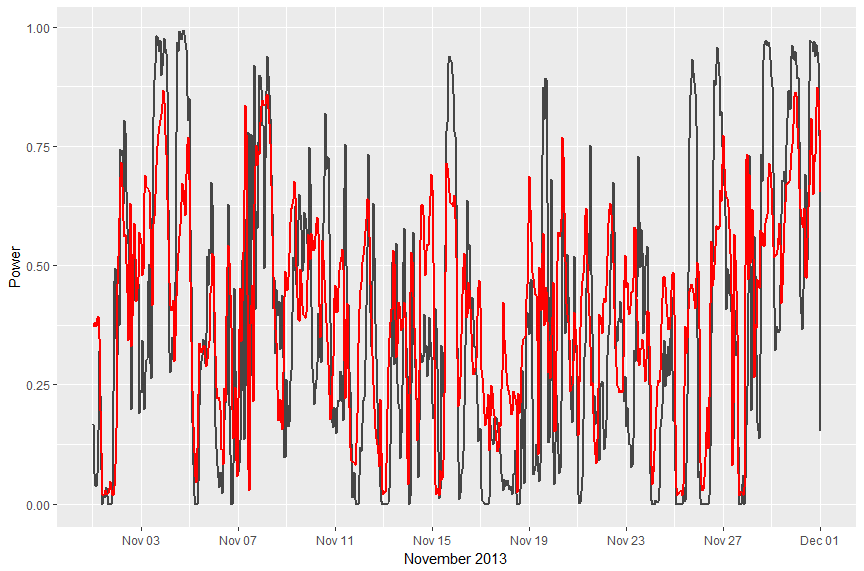
\includegraphics[scale=0.3, width=\textwidth]{figures/Rplot_ANN.png}\\[1cm]    
	\end{center}
	
	\subsection{Comparing prediction results of machine learning techniques}
	    For our comparative analysis, we are to consider the error function RMSE which is described by the formulation
	    
	   \begin{equation}
	        RMSE = \sqrt{\frac{1}{N}\sum_{i = 1}^{N}(y^{p}_{i} - y_{i})^2}.
	   \end{equation}
	    
	    Where $y^{p}$ is the predicted values and $y$ is the actual values \cite{rmseForm}. The accuracy of the predictions from the model is determined by this error function. A corollary to this is that we have a method to determine the cost and stability of wind power. When determining the accuracy of the models it is equally important to consider the context and use of the data. To be able to have a fair comparative, the data should be normalized and validated by the same methods. In our case we have chosen to use \emph{cross-validation} and test every model on the whole training set. Hence, the results.
        
    \begin{table}[!h]
        \centering
        \begin{tabular}{|c|c|c|c|c|}
            \hline
            & LR & KNN & SVM (regression) & ANN \\
            \hline
            RMSE & 0.2163841 & 0.2216553 & 0.2147279 & 0.2166363226 \\
            \hline
        \end{tabular}
        \caption{RMSE results from each run of the model}
        \label{LR_KNN_SVR_ANN_RMSE_results}
    \end{table}
        
        We can see from the table that the model with the lowest RMSE is the SVM model. When considering a SVM model it is important to consider its tendencies to over-fitting the training data. Usually, the model of SVM will be more generalized after being exposed to large training data sets. As mentioned earlier, this also occurs within the ANN model. When regarding how KNN evaluates the training data set, then it is important to know that finding the optimal $k$ value is what determines a valid model. As the K value increases, the prediction will often lead to a over-fitting problem and the model will be generalized. Lastly, linear regression is a model which is least likely to be prone to an over-fitting problem, since the  model considers a general mean between every single data point within the prediction. It is however a poor model for determining extreme data such as antipodal data. A model which is to be considered a valid model must determine the accuracy of the prediction such that it minimizes the over-fitting and generalization of the data. Therefore, the validity of SVM and ANN can be considered poor if it is exposed to large quantities of training data. In our case, we are to consider 16080 data points and to determine if these models are valid based on the data would require even further in depth analysis. However this would be considered outside the scope of this assignment. Although we have given a brief justification in the introduction.
        
        
    % \noindent Each method has a different training model.
    
    % \noindent We are to only consider 11.2013.
    
    % \noindent Save the predicted forecasts as ForecastTemplate-LR.csv, ForecastTemplate-kNN.csv, etc.
    
    % \noindent Finally, evaluate the prediction accuracy. Compare the forecasted wind power with the actual wind power 
    % by the use of the error metric RMSE.
    
    % Introduce the use of the "caret" library. Describe the use of it and what parameters to the different models needed to be tweaked to get the wanted optimization (hyperparameters).
    
    
\section{Question 2}
	

\subsection{Multiple Linear Regression}

    The general formulation of a multiple linear regression problem is
    
    \begin{equation}
        y_{p} = \beta_{1}x_{1} + \beta_{2}x_{2} + ... + C
    \end{equation}
    
    which is similar to the LR model, but may take multiple variables into consideration. In our case the formula would be
    
    \begin{equation}
        y_{p} = \beta_{1} \times Wind\ speed + \beta_{2} \times Wind\ direction + C
    \end{equation}
    
    where $\beta_{1} = 1.235e-01$, $\beta_{2} = -6.966e-05$ and $C = -7.463e-02$, after training the model on 16080 data points from the training data. We determine the \emph{wind direction} by
    
    \begin{equation}
        Wind\ direction = (270 - atan_{2}(V10,U10) \times \frac{180}{\pi})\ \%\ 360
    \end{equation}
	
 	where $V10$ and $U10$ is the data from the training and validation set, known as \emph{training\_data} and \emph{weather\_forecast\_input}, and the formula is given in \cite{winddir}. The symbol "\%" in this case refers to the arithmetic function \emph{modulo}. When considering what may generate wind power, it is important to understand that it may not only depend on wind speed, but multiple variables such as temperature, wind direction and pressure. Below is the provided accuracy results from running our model on the two variables mentioned in the formulation above.
 	
 	
 	\begin{table}[!h]
        \centering
        \begin{tabular}{|c|c|c|}
            \hline
             & LR & MLR \\
            \hline
            RMSE & 0.2163841 & 0.2149417 \\
            \hline
        \end{tabular}
        \caption{RMSE from LR and MLR model}
        \label{LR_MLR_RMSE_results}
    \end{table}
 	
    As for the figure below, we have that black is the MLR model, red is the LR model and green is the actual wind power for the time period.
    
\newpage

    \begin{center}
        \textbf{MLR prediction}\\
	    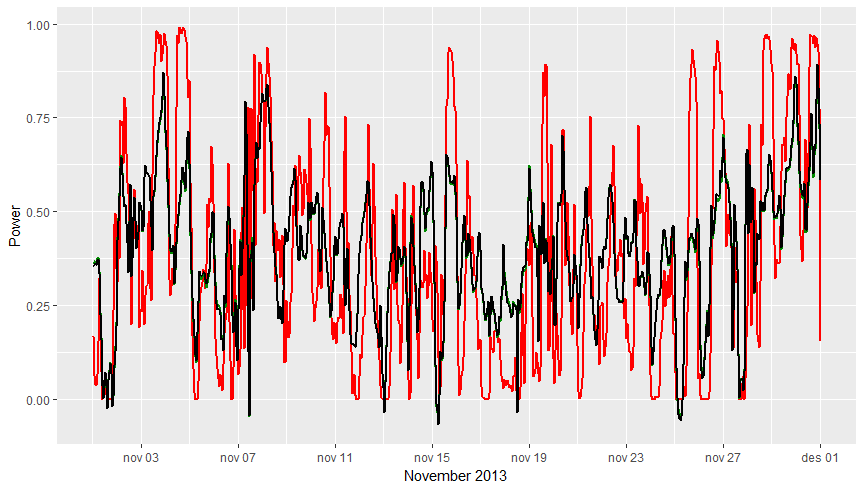
\includegraphics[scale=0.3, width=\textwidth]{figures/Rplot_MLR.png}\\[1cm]
    \end{center}
    
    Regarding the figure, it can be obscure which of the models are closest related to the actual wind power, but from the table above we can see that the MLR model outperformed the LR model. The reason for this is that by using multiple variables it may increase the prediction accuracy for wind power, and in our case we can see that wind direction has a positive effect on the accuracy estimation of the wind power. Furthermore, if we also considered temperature and pressure, for example, we could estimate the accuracy of the wind power on a granular level. Providing us with ideal conditions to have a valid model for estimating the accuracy of the wind power.
	
\section{Question 3}
    
    When considering the formulation, from lecture \cite{rnnLec}, it provides the necessary description of the problem, but may require additional intuition to grasp the concept of recurrent neural networks, also known as RNN. In Richard Socher's lecture notes \cite{rnnForm} we have found a simple RNN formulation:
    
   %When considering the formulation from the lecture \cite{rnnLec}, it provides the necessary description of the problem, but may require a generalization to better grasp the intuition of the recurrent neural network, also known as RNN, model. In Richard Socher's lecture notes \cite{rnnForm} we have found a simple RNN formulation:
    
    \begin{equation}
        \begin{split}
        h_{t} & = Wf(h_{t-1}) + W^{(hx)}x_{[t]} \\
        y_{t}^{p}  & = W^{(S)}f(h_{t})
        \end{split}
    \end{equation}
    
    In our formulation, we would replace $x$ with the wind power, which we can denote as $wind^{p}$. Where we are concerned with relating the hidden layer state $h_{t}$ with its past layer state $h_{t-1}$, as described in the lecture notes \cite{rnnLec}. Also, the hidden state $h_{t}$ is calculated based on the previous hidden state $h_{t-1}$ and the input $wind^{p}_{t}$ at the current time step. When considering the output $y_{t}^{p}$ it is calculated based on the memory $h_{t}$ at time $t$.
    
    For our RNN model we were required to partition the training data into two segments, since we were to provide a prediction of power based on power. The first partition was used to train the RNN model with 15000 of the first data points from the training data. As for the remaining data points, they were used to predict the power. The reason for separating the data in such a way is because we may not always have other forms of weather data available such as wind speed, temperature, pressure and wind direction. Our RNN model was heavily inspired by the RNN model provided from the lecture notes in \cite{rnnCode}. We were to compare our RNN model with a LR model which partitioned the data in a similar fashion. It provided us with the follow accuracy results:
   
    
    \begin{table}[!h]
        \centering
        \begin{tabular}{|c|c|c|}
            \hline
             & LR & RNN \\
            \hline
            RMSE & 0.4792255 & 0.4725564 \\
            \hline
        \end{tabular}
        \caption{RMSE from LR and RNN model}
        \label{LR_RNN_RMSE_results}
    \end{table}
    
    Finally, we were to plot a figure of the power prediction of the RNN and LR model with the actual power. We have that red is the RNN model, blue is the LR model and grey is the actual wind power for the time period.
 
    
    \begin{center}
        \textbf{RNN \& LR prediction}\\
	    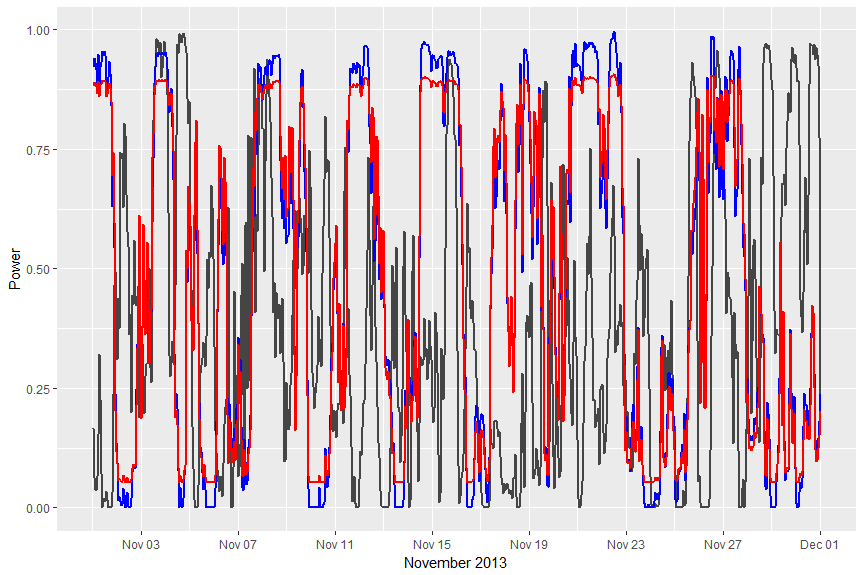
\includegraphics[scale=0.3, width=\textwidth]{figures/Rplot_RNN.png}\\[1cm]
    \end{center}

\section{Few final regards}
    Caret, the library used to implement the machine learning techniques, from the assignment, made it simple for anyone with prior statistical knowledge to use it without proficient programming abilities. For a computer science student, the black box, or abstraction, over the machine learning functions may cause a lack of understanding of the underlying mathematics. Especially, when wanting to understand the formulations underpinning the machine learning techniques from the assignment. If one is to fine tune the parameters to their optimal performance, then it requires \emph{a priori} knowledge of the algorithms and an in depth understanding of the context it may be applied.
    
\appendix
    
    % Hello, 
    %First, the minimum you have to do is that you present your results with random selection of the parameters.
    %Then, if you have more time, you can attempt to find an optimal value of the parameter.
    %It is better you provide the formulation.
    %If you have the formulation, you can compare the parameter selection in the report.

\section{File structure}
	    
	\subsection{File structure}
	    
	    Regarding our files the structure is as follows:
	    
	    \begin{enumerate}
	        \item data - contains both the test data and the output from the weather forecast predictions.
	        \item documents - contains the report.
	        \item figures - contain the plots from the assignment.
	        \item R - contains the code files: aNN.R, kNN.R, LR.R, MLR.R, RNN.R and SVR.R.
	    \end{enumerate}
	 
	    The file structure of the assignment where the R project is located is as following.
	    \begin{enumerate}
	        \item /Assignment 2/Machine learning/Weather Forecast/Weather Forecast.Rproj.
	    \end{enumerate}
	    
	    Question 1 is divided into 4 different files, aNN.R, kNN.R, SVR.R, LR.R.
	    
	    Question 2 only has 1 file called MLR.R. Here we solve multiple linear regression and then just use the same code for linear regression as used in question 1 LR.R. Thus, plotting a figure with three curves.
	    
	    Question 3 has also only one file called RNN-LR3.R
	    
	    Predicted forecast data we compile under the run of the code is in the folder predicted forecast which can be found in the folder called -data.
        
    \section{How to run the program}
        
        To be able to run most of the code you will have to install the packages correctly; caret, rnn and neuralnet. We have done it so that it gets installed automatically when ran, but there might be some slight hiccups.
        
        Open the "Weather Forecast.Rproj" file in RStudio. To execute the line of source code where the cursor currently resides you press the Ctrl+Enter key (or use the Run toolbar button). To run the entire document press the Ctrl+Shift+Enter key (or use the Source toolbar button), and press "Run" in R.

\newpage

    \printbibliography[heading=bibintoc]
\end{document}
